% One big task, or a series of small ones with a review point between each.
% ---------------------------------------------------------------------------
% style.tex --- shared preamble for every figure in book/figures/tikz/
%
% One style for all figures: Latin Modern, thin black lines, a light grey
% fill, and one accent colour used only to mark what is untrusted or wrong.
% Build with scripts/build_figures.sh; see book/figures/README.md.
% ---------------------------------------------------------------------------
\documentclass[tikz,border=6pt]{standalone}
\usepackage[T1]{fontenc}
\usepackage{lmodern}
\usetikzlibrary{arrows.meta,positioning,shapes.geometric,calc,fit,backgrounds}

\hyphenpenalty=10000   % short lines in boxes: ragged, never hyphenated

\definecolor{lightgrey}{gray}{0.92}
\definecolor{accent}{HTML}{9B2D20}

\tikzset{
  every picture/.style={
    line width=0.6pt,
    font=\small,
    >={Stealth[length=5pt,width=4pt]},
    node distance=14pt and 24pt,
  },
  % shapes
  box/.style={draw, rectangle, inner xsep=8pt, inner ysep=5pt,
              minimum height=22pt, align=center},
  grey/.style={box, fill=lightgrey},
  rounded/.style={box, rounded corners=9pt},
  decision/.style={draw, diamond, aspect=2.4, inner sep=1.5pt, align=center},
  group/.style={draw, dashed, rounded corners=5pt, inner sep=7pt},
  % text
  tag/.style={font=\footnotesize, align=center, inner sep=2pt},
  note/.style={font=\footnotesize\itshape, align=center, inner sep=2pt},
  code/.style={font=\small\ttfamily},
  codetag/.style={font=\footnotesize\ttfamily, align=center, inner sep=2pt},
  title/.style={font=\small\scshape, align=center, inner sep=2pt},
  % lines
  arrow/.style={->},
  back/.style={->, dashed},
  thin/.style={line width=0.4pt, gray},
  % the one accent, for what is untrusted, wrong or missing
  bad/.style={accent},
  badbox/.style={box, draw=accent, text=accent},
}

\begin{document}
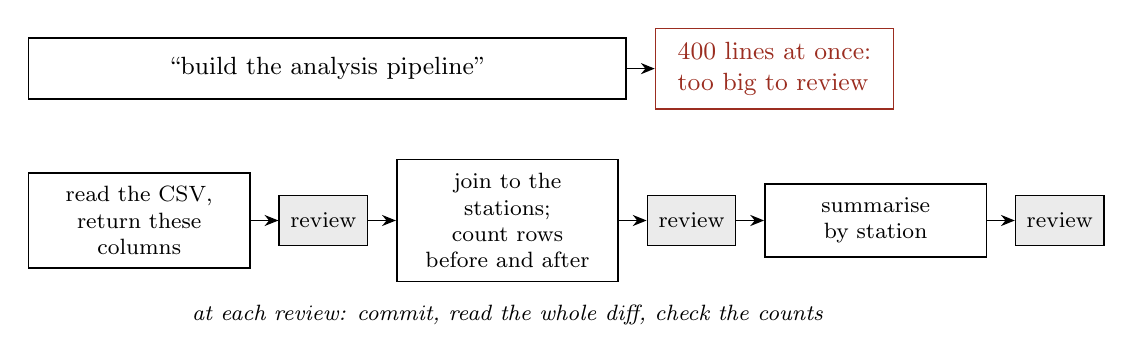
\begin{tikzpicture}[node distance=10pt and 10pt,
                    rev/.style={grey, font=\footnotesize, inner xsep=4pt, minimum height=18pt},
                    small/.style={box, text width=64pt, font=\footnotesize}]
  \node[box, text width=200pt] (big) {``build the analysis pipeline''};
  \node[badbox, right=of big, align=left] (out) {400 lines at once:\\too big to review};
  \draw[->] (big) -- (out);

  \node[small, below=26pt of big.south west, anchor=north west] (s1) {read the CSV,\\return these columns};
  \node[rev, right=of s1] (r1) {review};
  \node[small, right=of r1] (s2) {join to the stations;\\count rows before and after};
  \node[rev, right=of s2] (r2) {review};
  \node[small, right=of r2] (s3) {summarise\\by station};
  \node[rev, right=of s3] (r3) {review};
  \draw[->] (s1) -- (r1); \draw[->] (r1) -- (s2);
  \draw[->] (s2) -- (r2); \draw[->] (r2) -- (s3);
  \draw[->] (s3) -- (r3);
  \node[note, below=6pt of s2.south, anchor=north] {at each review: commit, read the whole diff, check the counts};
\end{tikzpicture}
\end{document}
